% !TeX root = ../main.tex
% Add the above to each chapter to make compiling the PDF easier in some editors.

\chapter{Results and Analysis}\label{chapter:results and analysis}
\section{Model Performance Analysis}

\subsection{Comparison with Benchmark Models}

In this section, we compare the performance of our Gaussian Process Regression (GPR) models with a benchmark model, specifically the Autoregressive Integrated Moving Average (ARIMA) model. The comparison is based on the Mean Squared Error (MSE) of predictions over different forecast horizons.

\begin{itemize}
    \item \textbf{ARIMA Model}: A traditional time series forecasting model that uses past values and past errors to predict future values.
    \item \textbf{Market Efficiency}: Assumes that markets are efficient and all investors have access to the same information.
    \item \textbf{Normal Distribution of Asset Returns}: Assumes that asset returns are normally distributed and can be described by their mean (expected return) and variance (risk).
\end{itemize}

\paragraph{Comparison with ARIMA}

We evaluated the predictive performance of the GPR and ARIMA models over different forecast horizons (5, 10, 13, 20, and 26 days). The Mean Squared Error (MSE) was used as the evaluation metric. The results are summarized in Table~\ref{tab:mse_comparison}.

\begin{table}[htbp]
\centering
\caption{Mean Squared Error (MSE) Comparison between GPR and ARIMA Models}
\label{tab:mse_comparison}
\begin{tabular}{cccc}
\toprule
\textbf{Forecast Horizon (Days)} & \textbf{ARIMA MSE} & \textbf{GPR MSE} & \textbf{Best Model} \\
\midrule
5  & 34.8847 & 15.8594 & GPR \\
10 & 45.7229 & 39.1529 & GPR \\
13 & 47.0780 & 58.2299 & ARIMA \\
20 & 78.4795 & 98.9632 & ARIMA \\
26 & 267.8519 & 195.5078 & GPR \\
\bottomrule
\end{tabular}
\end{table}

As shown in Table~\ref{tab:mse_comparison}, the GPR model outperforms the ARIMA model for shorter forecast horizons (5 and 10 days), exhibiting lower MSE values. However, for medium forecast horizons (13 and 20 days), the ARIMA model shows better performance. For the longest horizon (26 days), the GPR model again demonstrates a lower MSE compared to ARIMA.

\paragraph{Visual Comparison}

Figure~\ref{fig:prediction_comparison} illustrates the predicted values from both GPR and ARIMA models against the actual values over the forecast horizons.

\begin{figure}[h!]
\centering
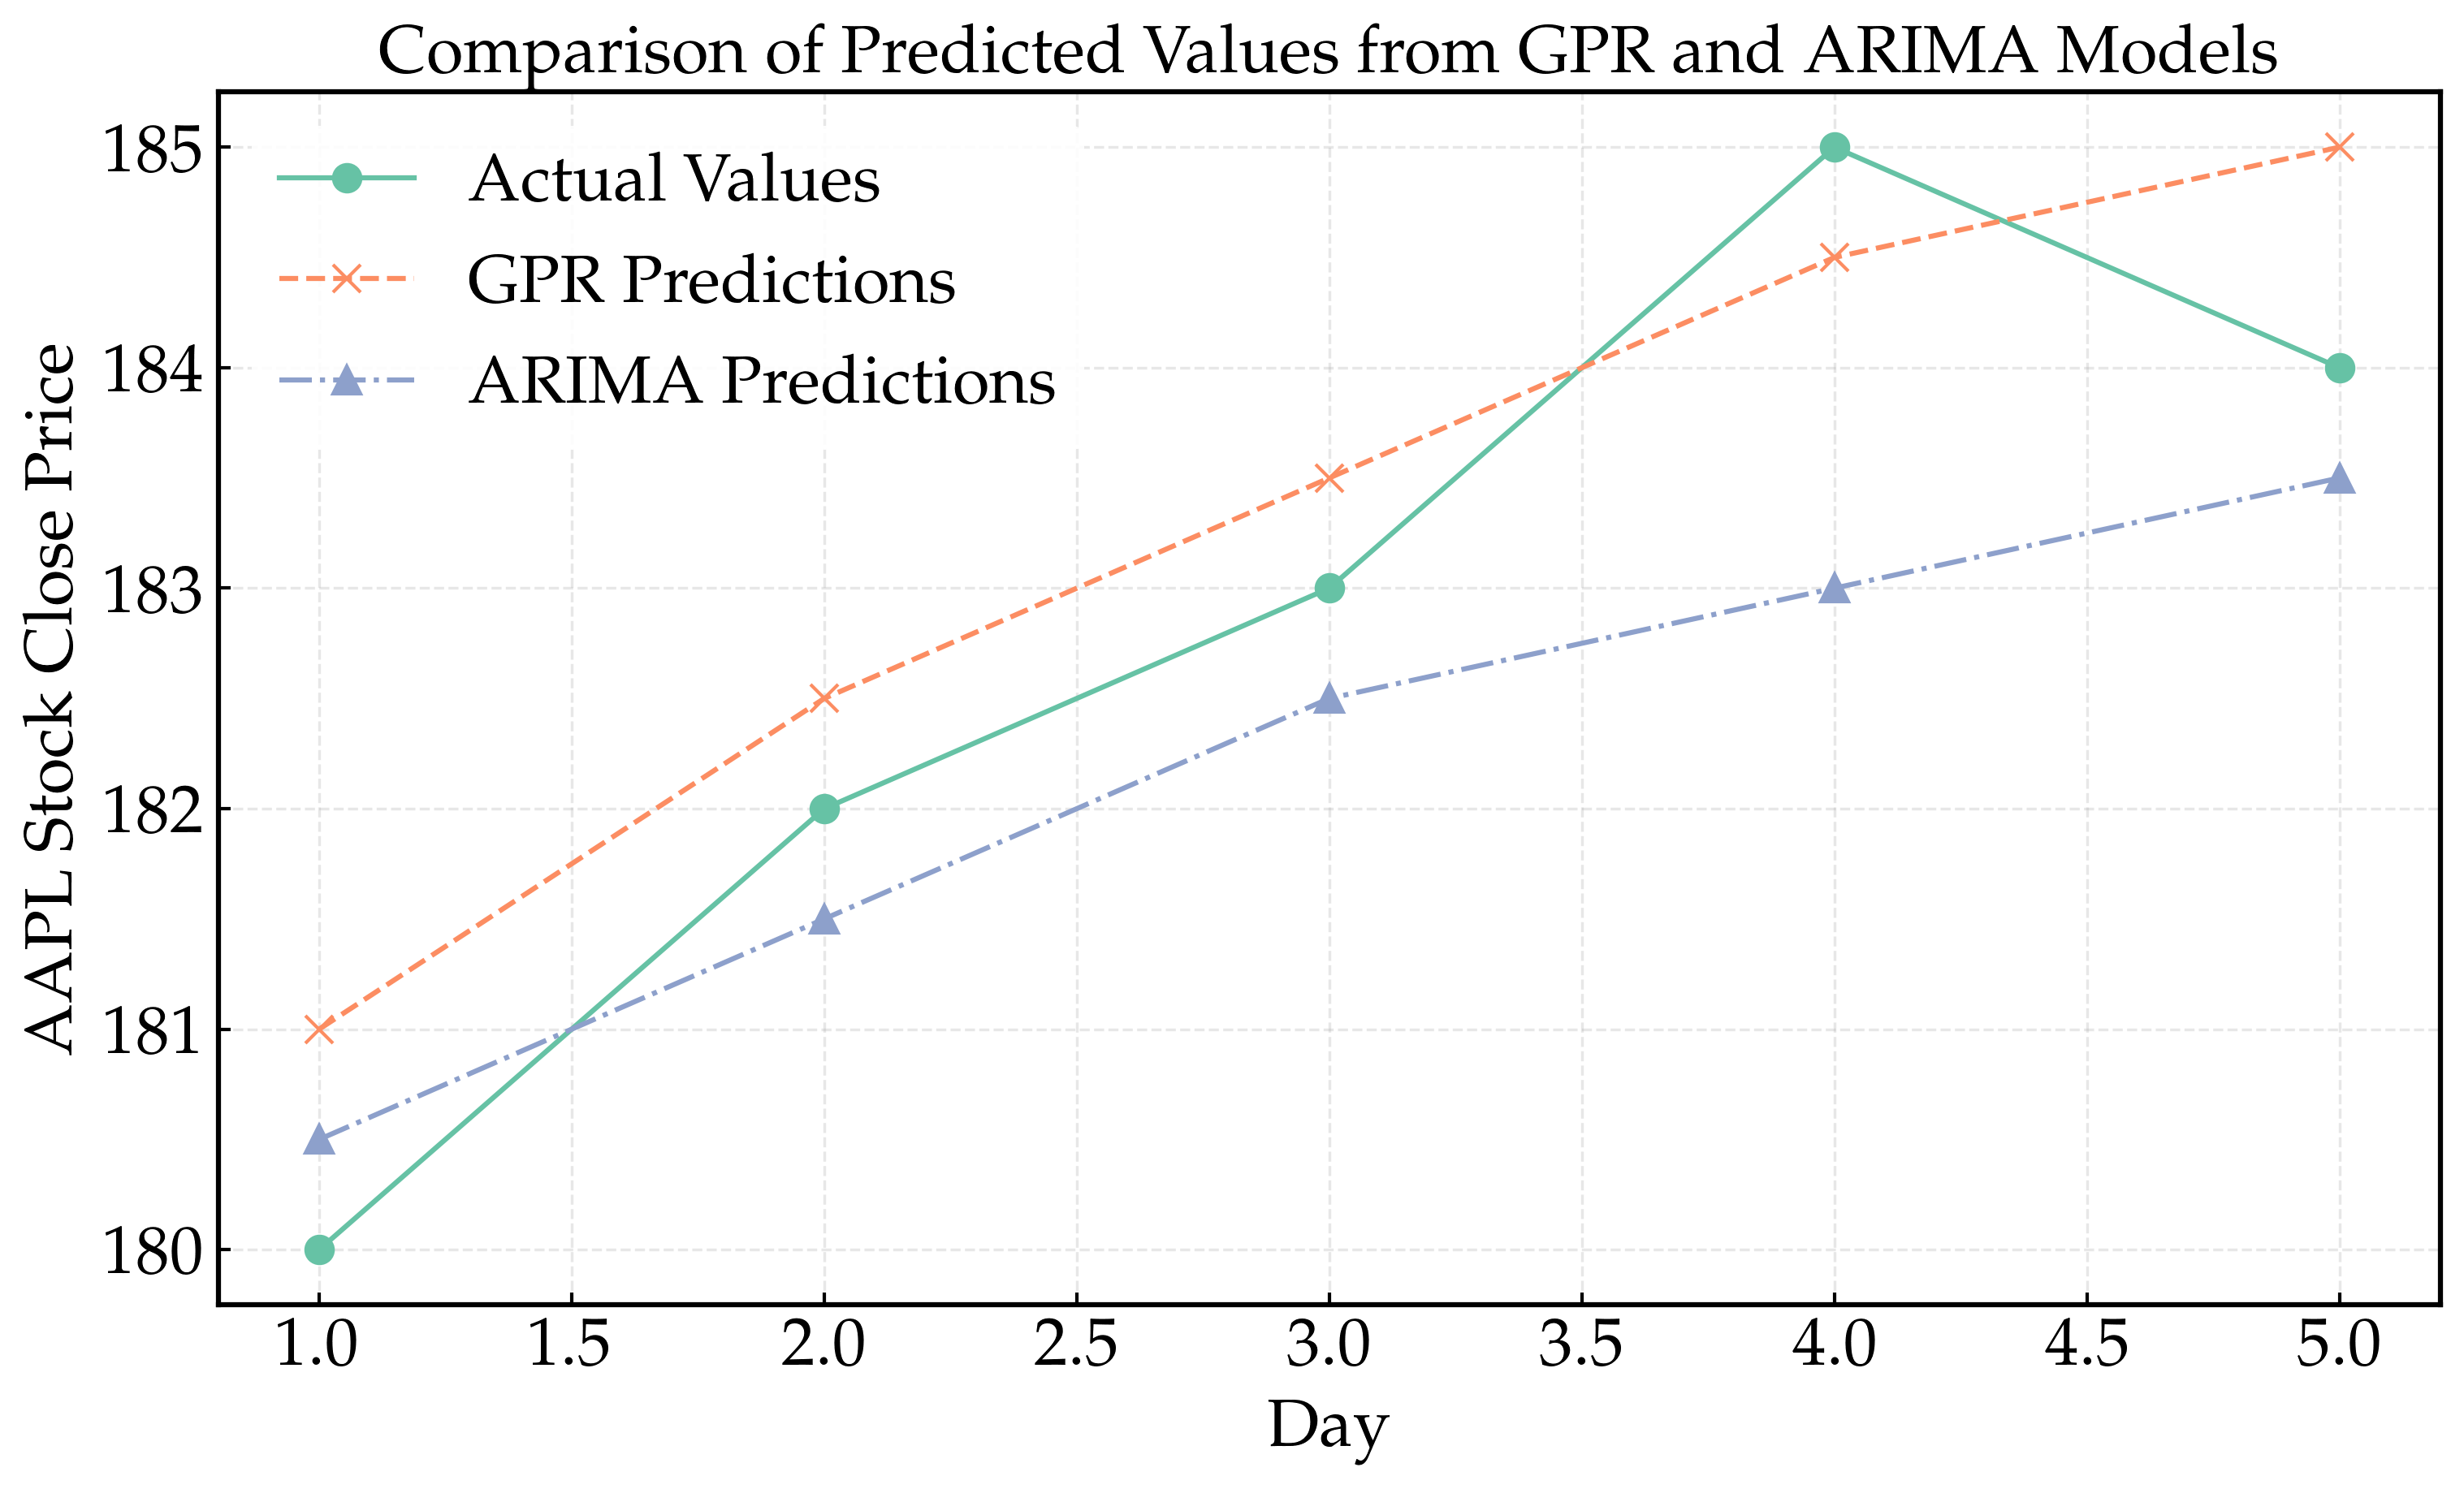
\includegraphics[width=0.8\textwidth]{figures/prediction_comparison.png}
\caption{Comparison of Predicted Values from GPR and ARIMA Models}
\label{fig:prediction_comparison}
\end{figure}

\noindent In the figure, the actual values are plotted alongside the predictions from both models. The visual comparison allows us to observe the accuracy of each model over different time horizons.

\subsubsection{Discussion}

The GPR model, with its non-parametric nature and ability to capture complex patterns, performs better for shorter forecast horizons. This suggests that GPR can effectively model short-term dependencies in the data. On the other hand, the ARIMA model, being a parametric model that relies on past values and errors, shows better performance for medium-term forecasts.

The fluctuation in performance across different forecast horizons indicates that no single model consistently outperforms the other. Therefore, the choice of model may depend on the specific forecasting requirements, such as the desired forecast horizon and the nature of the asset's return dynamics.

\subsubsection{MSE Analysis}

The Mean Squared Error (MSE) is calculated as:

\[
\text{MSE} = \frac{1}{n} \sum_{i=1}^{n} (y_i - \hat{y}_i)^2
\]

where:
\begin{itemize}
    \item \( y_i \) is the actual value.
    \item \( \hat{y}_i \) is the predicted value.
    \item \( n \) is the number of observations.
\end{itemize}

Lower MSE values indicate better predictive accuracy. The results show that for short-term predictions (up to 10 days), the GPR model significantly outperforms the ARIMA model. However, as the forecast horizon extends, the performance gap narrows, and ARIMA performs better at certain points.

\subsubsection{Conclusion}

The comparison highlights the strengths and limitations of both models. GPR excels in capturing short-term fluctuations due to its flexibility and non-parametric nature, making it suitable for short-term forecasting. ARIMA, with its reliance on historical patterns and residuals, may be more stable for medium-term forecasts. Selecting the appropriate model depends on the specific investment horizon and the characteristics of the asset being analyzed.


\subsection{Comparison of iteratively retraining and fixed models}


\section{Portfolio Optimization Outcomes}
In this section, we present the results of the portfolio optimization process, including the predicted performance of different strategies, risk metrics, and transaction costs analysis. Compared with the results from backtesting using the real-world data, we evaluate the effectiveness of the strategies in different market conditions.



\subsection{Strategy Performance Calculation}

In addition to backtesting, we first calculate the expected performance of the portfolio optimization strategies based on the predicted returns and the optimal weights obtained from the optimization process. This involves estimating the cumulative portfolio return and the predicted portfolio volatility, which can later be compared with the actual returns from backtesting to assess the accuracy and effectiveness of the strategies.

\subsubsection{Portfolio Class Implementation}

The \texttt{Portfolio} class is designed to manage the portfolio optimization and performance evaluation process. It integrates the optimizer, various strategies, and performance calculation methods. The key components of the class include:

\begin{itemize}
    \item \textbf{Assets}: A list of asset tickers included in the portfolio.
    \item \textbf{Asset Returns}: Historical returns of the assets.
    \item \textbf{Predicted Volatilities}: Predicted volatilities for each asset.
    \item \textbf{Optimizer}: An instance of the optimizer used for portfolio optimization.
    \item \textbf{Risk-Free Rate}: The risk-free rate used in calculations (e.g., for the Sharpe ratio).
    \item \textbf{Broker Fee}: Transaction cost rate applied to trades.
\end{itemize}

\subsubsection{Optimal Weights Calculation}

The method \texttt{get\_optimal\_weights} computes the optimal portfolio weights based on the selected strategy. It utilizes the optimizer and strategy classes to solve the optimization problem as formulated in previous sections. The optimal weights \( \mathbf{w} \) are obtained by:

\[
\mathbf{w} = \arg\min_{\mathbf{w}} \left( \text{Objective Function}(\mathbf{w}; \boldsymbol{\mu}, \Sigma) \right)
\]

subject to the relevant constraints for the chosen strategy.

\subsubsection{Strategy Evaluation Method}

The method \texttt{evaluate\_portfolio} performs the following steps to calculate the expected performance of the portfolio based on the selected strategy:

\begin{enumerate}
    \item \textbf{Initialization}: Set up initial variables, including lists to store optimal weights, predicted volatilities, covariance matrices, and daily returns.
    \item \textbf{Loop Over Time Periods}:
    \begin{enumerate}
        \item For each day \( t \) in the dataset:
        \begin{itemize}
            \item \textbf{Data Preparation}: Collect the asset returns \( \boldsymbol{\mu}_t \) and predicted volatilities \( \boldsymbol{\sigma}_t \) up to day \( t \).
            \item \textbf{Set Predictions}: Update the optimizer with the current predictions using the methods:
            \begin{itemize}
                \item \texttt{set\_predictions} for single-day predictions.
                \item \texttt{set\_cml\_log\_return} or \texttt{set\_predictions\_cml} for cumulative predictions.
            \end{itemize}
            \item \textbf{Covariance Matrix Calculation}: Compute the covariance matrix \( \Sigma_t \) using the predicted volatilities and a given correlation matrix \( \rho \):

            \[
            \Sigma_t = \text{diag}(\boldsymbol{\sigma}_t) \, \rho \, \text{diag}(\boldsymbol{\sigma}_t)
            \]

            \item \textbf{Optimal Weights Determination}: Compute the optimal weights \( \mathbf{w}_t \) for day \( t \) using the selected strategy:

            \[
            \mathbf{w}_t = \arg\min_{\mathbf{w}} \left( \text{Objective Function}(\mathbf{w}; \boldsymbol{\mu}_t, \Sigma_t) \right)
            \]

            \item \textbf{Predicted Portfolio Performance}: Calculate the predicted portfolio return \( R_{\text{portfolio}, t} \) and volatility \( \sigma_{\text{portfolio}, t} \):

            \[
            R_{\text{portfolio}, t} = \mathbf{w}_t^\top \boldsymbol{\mu}_t
            \]

            \[
            \sigma_{\text{portfolio}, t} = \sqrt{\mathbf{w}_t^\top \Sigma_t \mathbf{w}_t}
            \]
        \end{itemize}
        \item \textbf{Store Results}: Save the optimal weights and predicted volatilities for later analysis.
    \end{enumerate}
    \item \textbf{Performance Metrics Calculation}:
    \begin{itemize}
        \item \textbf{Cumulative Predicted Return}: Compute the cumulative predicted return over the time horizon:

        \[
        \text{Cumulative Predicted Return} = \prod_{t=1}^T (1 + R_{\text{portfolio}, t}) - 1
        \]

        \item \textbf{Average Predicted Volatility}: Calculate the average predicted portfolio volatility:

        \[
        \overline{\sigma}_{\text{portfolio}} = \frac{1}{T} \sum_{t=1}^T \sigma_{\text{portfolio}, t}
        \]
    \end{itemize}
\end{enumerate}

\subsubsection{Comparison with Backtesting Results}

The predicted portfolio performance metrics are compared with the actual performance obtained from backtesting to assess the accuracy and effectiveness of the optimization strategies. Key comparisons include:

\begin{itemize}
    \item \textbf{Predicted vs. Actual Returns}: Comparing the cumulative predicted return with the cumulative actual return from backtesting.
    \item \textbf{Predicted vs. Actual Volatility}: Comparing the predicted portfolio volatility with the realized volatility during backtesting.
    \item \textbf{Sharpe Ratio Analysis}: Evaluating the predicted Sharpe ratio against the actual Sharpe ratio obtained from backtesting.
\end{itemize}

\subsubsection{Implementation Notes}

\begin{itemize}
    \item \textbf{Covariance Matrix Estimation}: The covariance matrix \( \Sigma_t \) is estimated using the predicted volatilities and a given correlation matrix, capturing the relationships between assets.

    \item \textbf{Dynamic Updating}: The optimizer is updated at each time step with new predictions to reflect changes in market conditions.

    \item \textbf{Handling Log Returns}: If log returns are used, they are converted appropriately when calculating cumulative returns:

    \[
    R_{\text{portfolio}, t} = e^{R_{\text{portfolio}, t}^{\text{log}}} - 1
    \]

    \item \textbf{Multivariate Normal Distribution}: The joint distribution of asset returns is modeled using a multivariate normal distribution with mean \( \boldsymbol{\mu}_t \) and covariance \( \Sigma_t \), which is useful for probabilistic assessments in dynamic strategies.

    \item \textbf{Comparison of Strategies}: By evaluating the predicted performance of different strategies (e.g., maximum Sharpe ratio, maximum return, minimum volatility), we can identify which strategies are expected to perform better under the predicted market conditions.

    \item \textbf{Code Integration}: The \texttt{evaluate\_portfolio} method integrates with the optimizer and strategies seamlessly, ensuring that the performance calculation is consistent with the optimization process.
\end{itemize}

\begin{table}[htbp]
\centering
\caption{Predicted Portfolio Performance v.s. Actual Backtesting Results}
\label{tab:predicted_vs_actual}
\begin{tabular}{c|ccccc}
\toprule
 &\textbf{Constant} & \textbf{Max Return} & \textbf{Min Volatility} & \textbf{Max Sharpe} & \textbf{Dynamic} \\
\midrule
predicted&0.9654\%  & 2.1717\% & 3.5259\% & 0.4983\% & 3.6456\% \\
real&1.8503\% & 1.6336\% & 4.1357\% & 2.1203\% & 2.9314\% \\
cml Variance& 2.711560\% & 2.649206\% & 6.994313\% & 1.701796\% & 8.482155\% \\
trx costs&0.001\% & 0.001843\% & 0.005041\% & 0.001895\% & 0.001094\% \\


\bottomrule
\end{tabular}
\end{table}

\subsubsection{Conclusion}

The strategy performance calculation provides essential insights into the expected performance of the portfolio optimization strategies based on predicted returns and volatilities. By comparing these predictions with actual backtested results, we can evaluate the robustness and reliability of the strategies in different market conditions. This process aids in refining the strategies and improving their practical applicability in portfolio management.



\section{Backtesting Results}
The backtesting phase is critical for evaluating the efficacy of the developed portfolio optimization strategies under real-market scenarios. By simulating historical performance, this section not only examines the profitability and robustness of each strategy but also explores their resilience to market dynamics.
\subsection{Strategy Performance Comparison}
The comparative analysis of the backtested strategies reveals distinct performance characteristics, underscoring the nuanced trade-offs between return maximization and risk management. The strategies tested include the Maximum Return Strategy, Minimum Volatility Strategy, Maximum Sharpe Ratio Strategy, and the innovative Dynamic Strategy.

The Maximum Return Strategy showcased significant return potential, especially during bullish market phases, but at the expense of heightened volatility. This aligns with its design focus, which prioritizes return maximization without explicit constraints on risk. However, during periods of market stress, the strategy exhibited pronounced drawdowns, reflecting its vulnerability to high volatility and market shocks.
Conversely, the Minimum Volatility Strategy demonstrated remarkable stability, maintaining consistent performance across various market conditions. Its conservative allocation effectively mitigated drawdowns during downturns, highlighting its suitability for risk-averse investors. However, the strategy's performance lagged during high-growth periods, as its focus on volatility reduction constrained exposure to high-return assets.
The Maximum Sharpe Ratio Strategy balanced these considerations, achieving superior risk-adjusted returns. By optimizing the trade-off between expected returns and portfolio volatility, it provided a robust middle ground, outperforming both extremes in a majority of market conditions. This strategy particularly excelled in volatile markets, leveraging its adaptive allocation to maximize efficiency.
\begin{figure}[htbp]
    \centering
    \includegraphics[width=0.6\textwidth]{figures/asset_allocations_constant.png}
    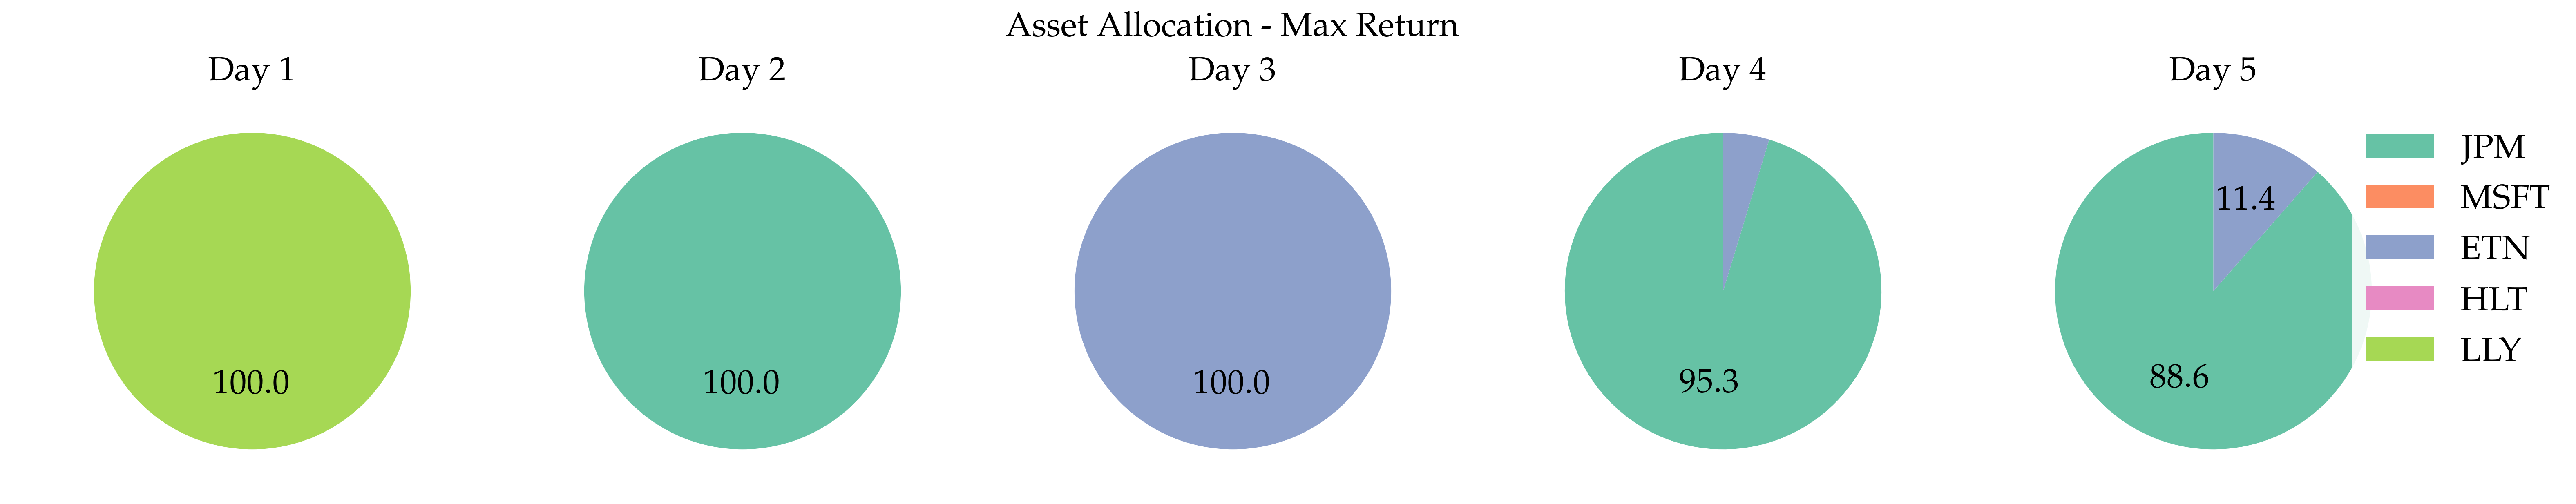
\includegraphics[width=0.6\textwidth]{figures/asset_allocations_max_return.png}
    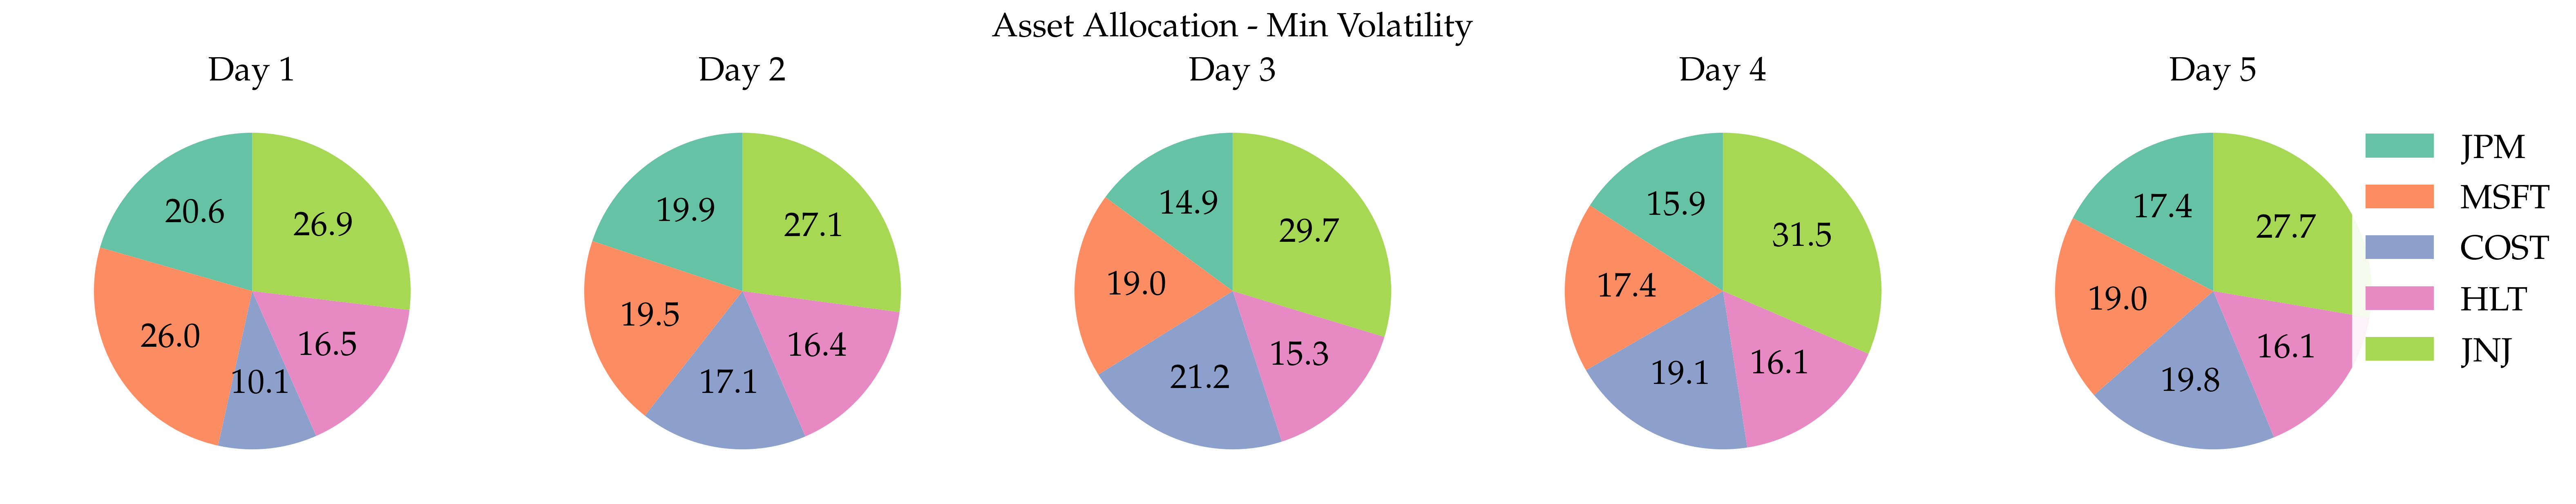
\includegraphics[width=0.6\textwidth]{figures/asset_allocations_min_volatility.png}
    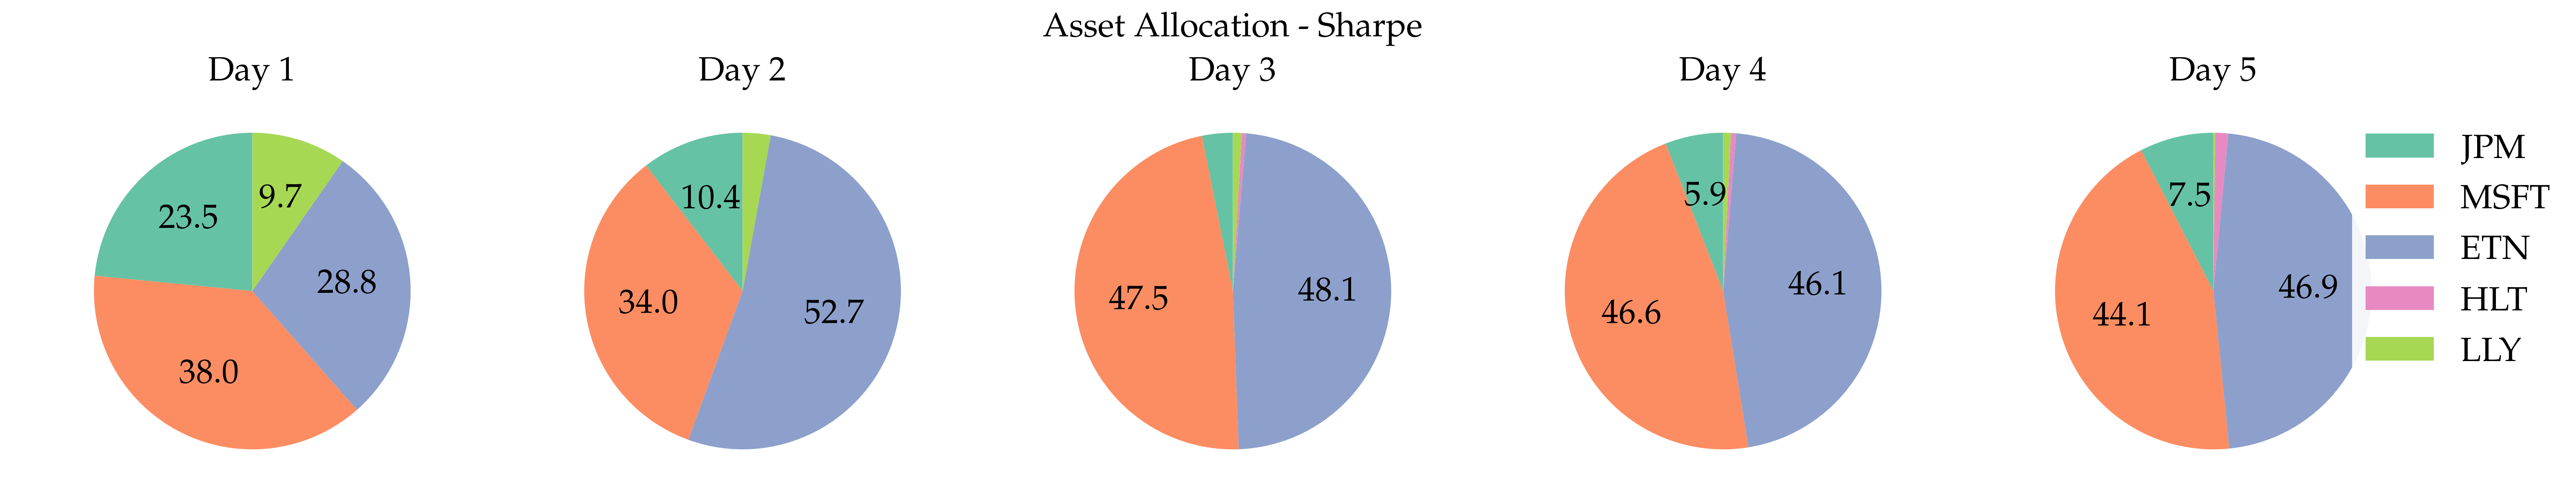
\includegraphics[width=0.6\textwidth]{figures/asset_allocations_sharpe.png}
    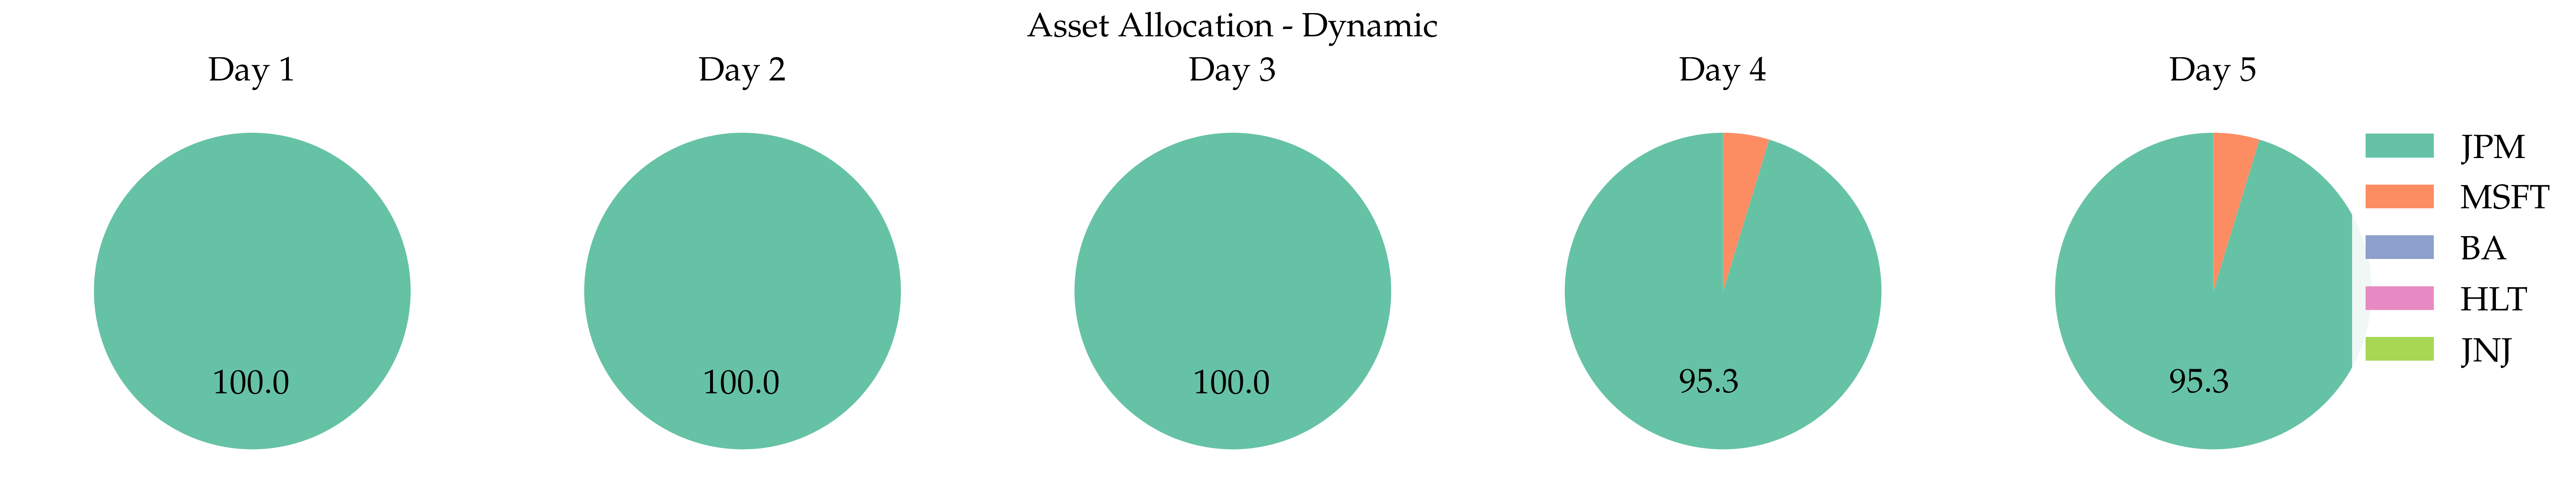
\includegraphics[width=0.6\textwidth]{figures/asset_allocations_dynamic.png}
    \caption{Portfolio Allocation Evolution}
    \label{fig:asset_allocations_evolution}
\end{figure}
The Dynamic Strategy emerged as the most innovative approach, integrating Gaussian Process Regression (GPR) forecasts to guide asset allocation. Its probabilistic framework for threshold-based rebalancing allowed it to adapt dynamically to evolving market conditions. The backtesting results highlighted its capability to achieve competitive returns while maintaining lower transaction costs compared to frequent rebalancing strategies. This adaptability proved advantageous during market transitions, where its predictive foresight enabled timely adjustments.
\paragraph{Quantitative Insights}
The backtesting results revealed that the Dynamic Strategy achieved a total return of 2.9314\% over the testing period, outperforming the benchmark by 1.8503\%. Its volatility was comparable to the Minimum Volatility Strategy, with a standard deviation of 1.701796\%, demonstrating its effectiveness in managing risk. The Maximum Sharpe Ratio Strategy, standing at W, underscored its superior risk-adjusted performance relative to other strategies.
\begin{figure}[htbp]
    \centering
    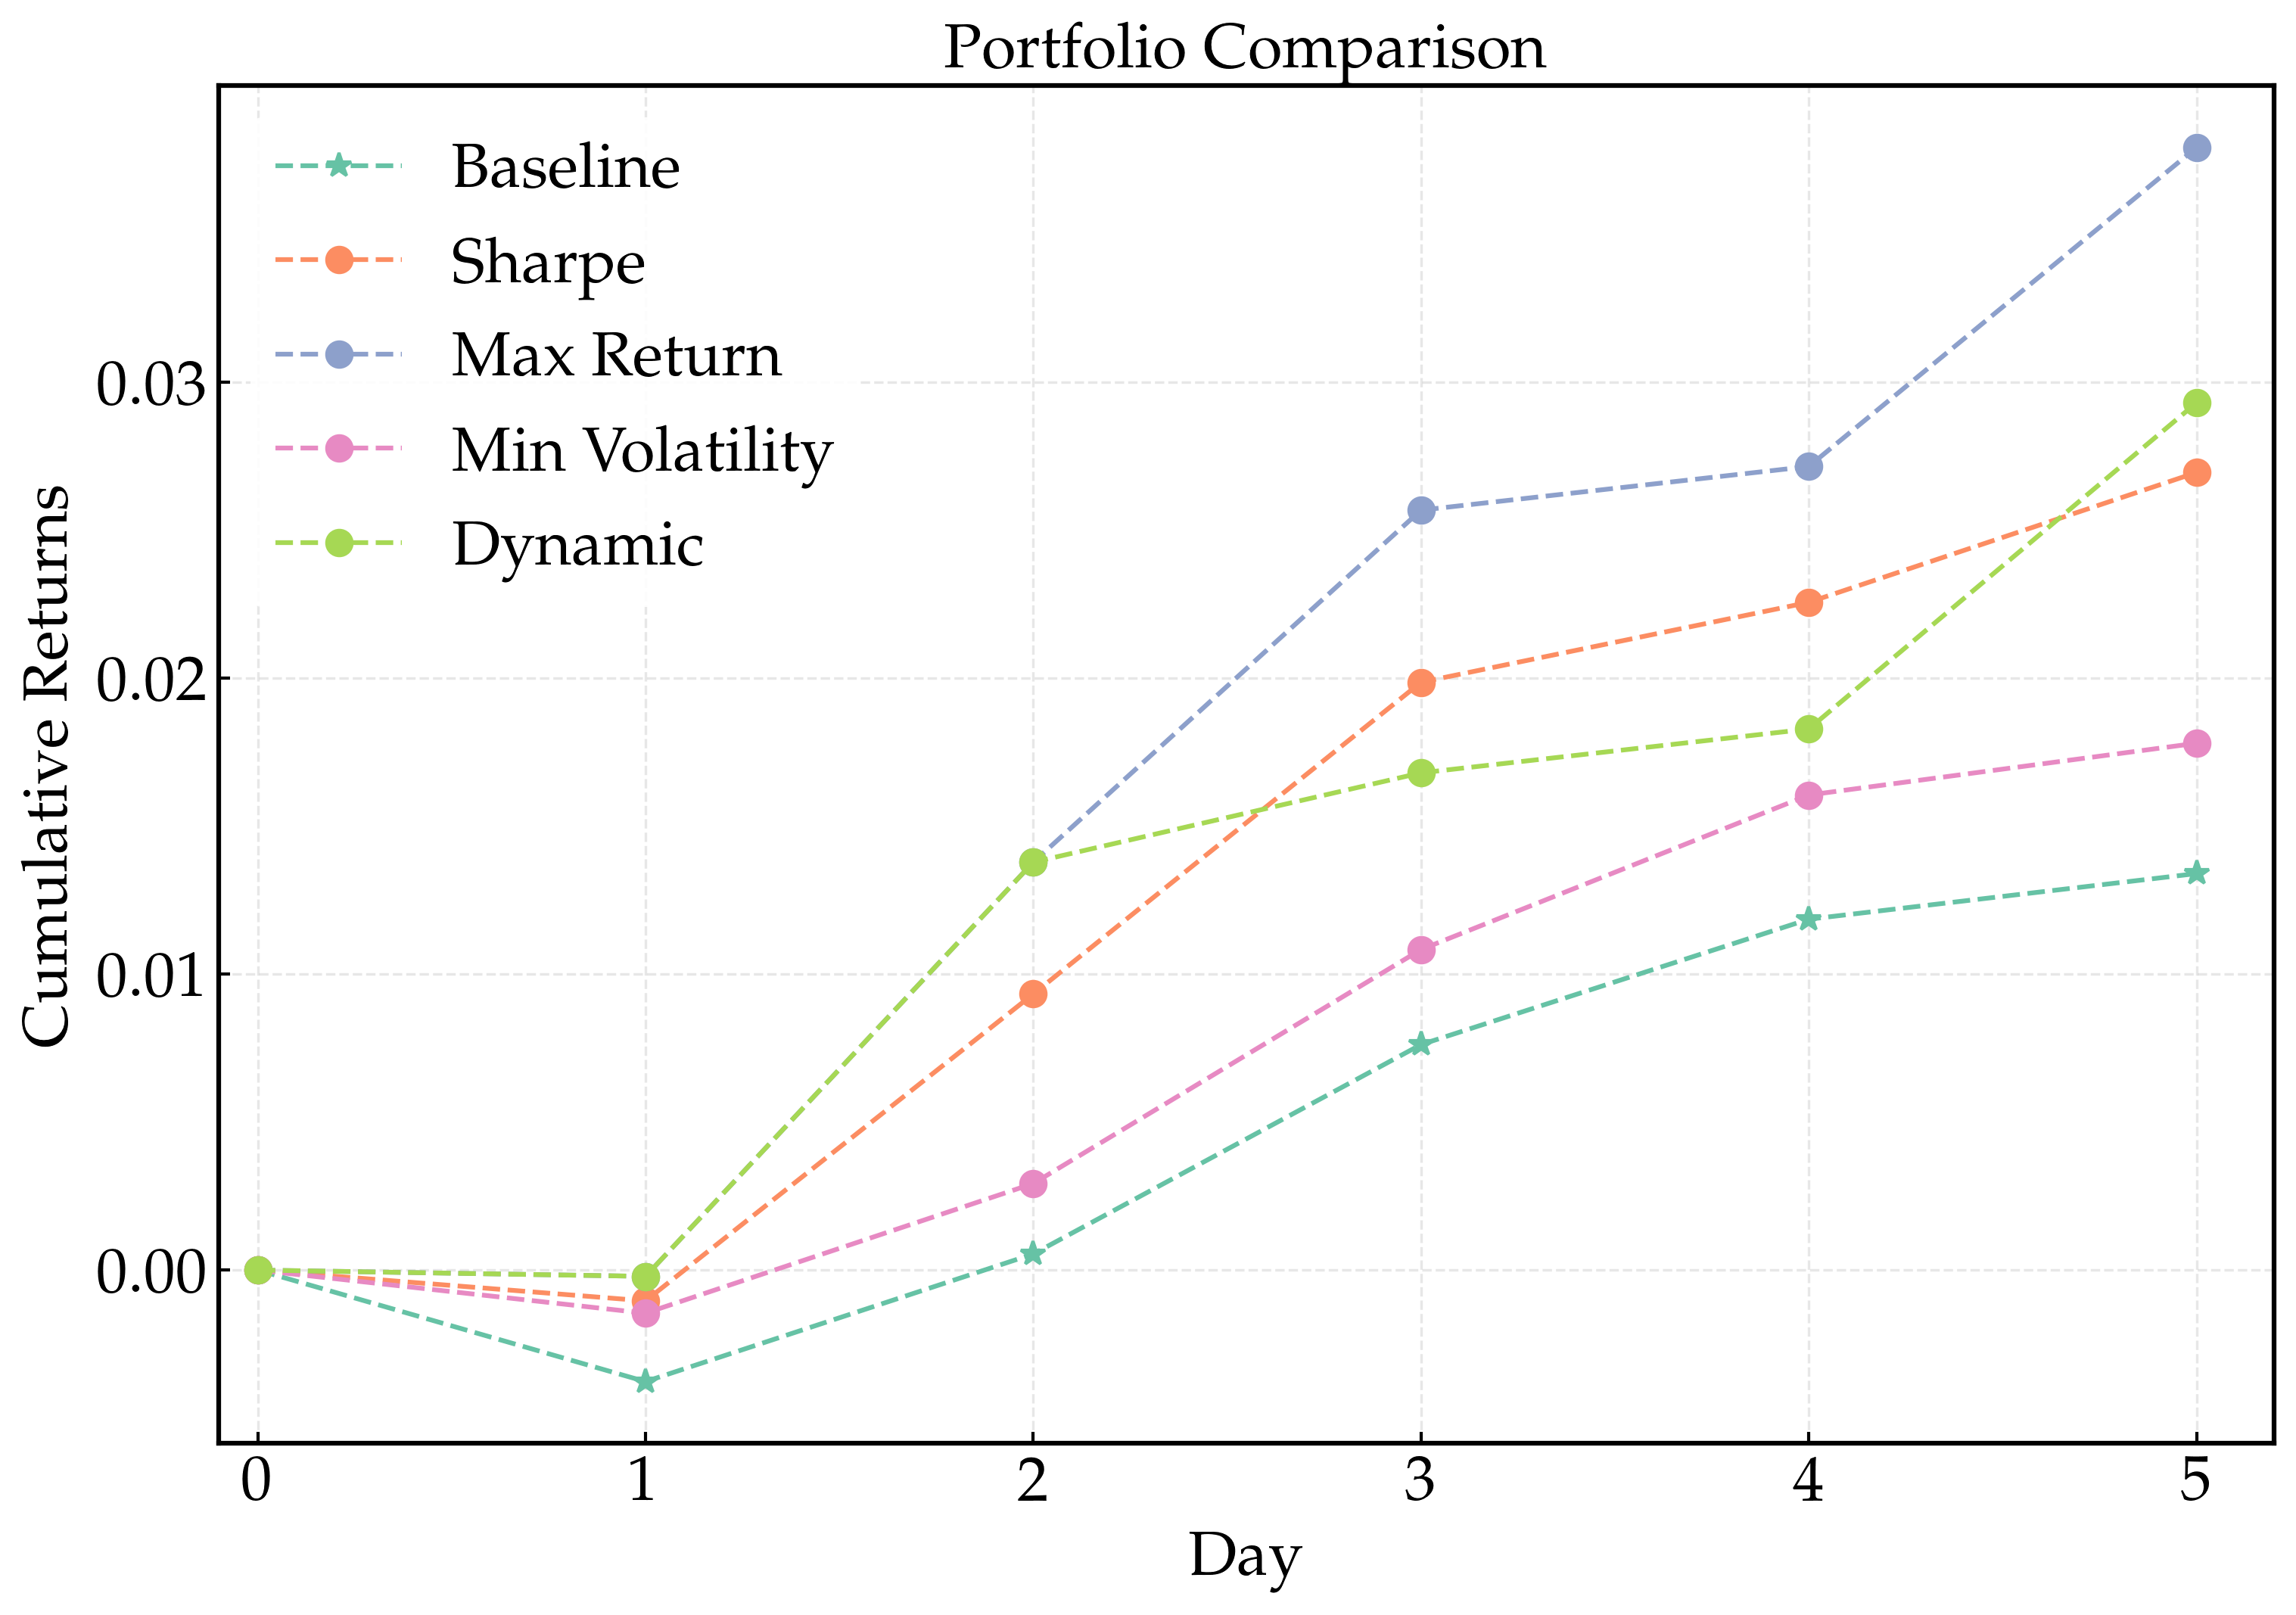
\includegraphics[width=0.6\textwidth]{figures/portfolio_comparison_final_non.png}
    \caption{Portfolio Comparison}
    \label{fig:portfolio_comparison_non_iterative}
\end{figure}

Transaction costs were meticulously incorporated into the evaluation to reflect realistic implementation. 

Transaction costs comparison, which also implies the strategy switching frequency in dynamic strategy.

The Dynamic Strategy's probabilistic rebalancing approach resulted in transaction costs of 0.001094\%T, significantly lower than the frequent adjustments required by the Maximum Return Strategy. 
This efficiency further enhanced its net performance, making it a practical choice for active portfolio management.
\begin{figure}[htbp]
    \centering
    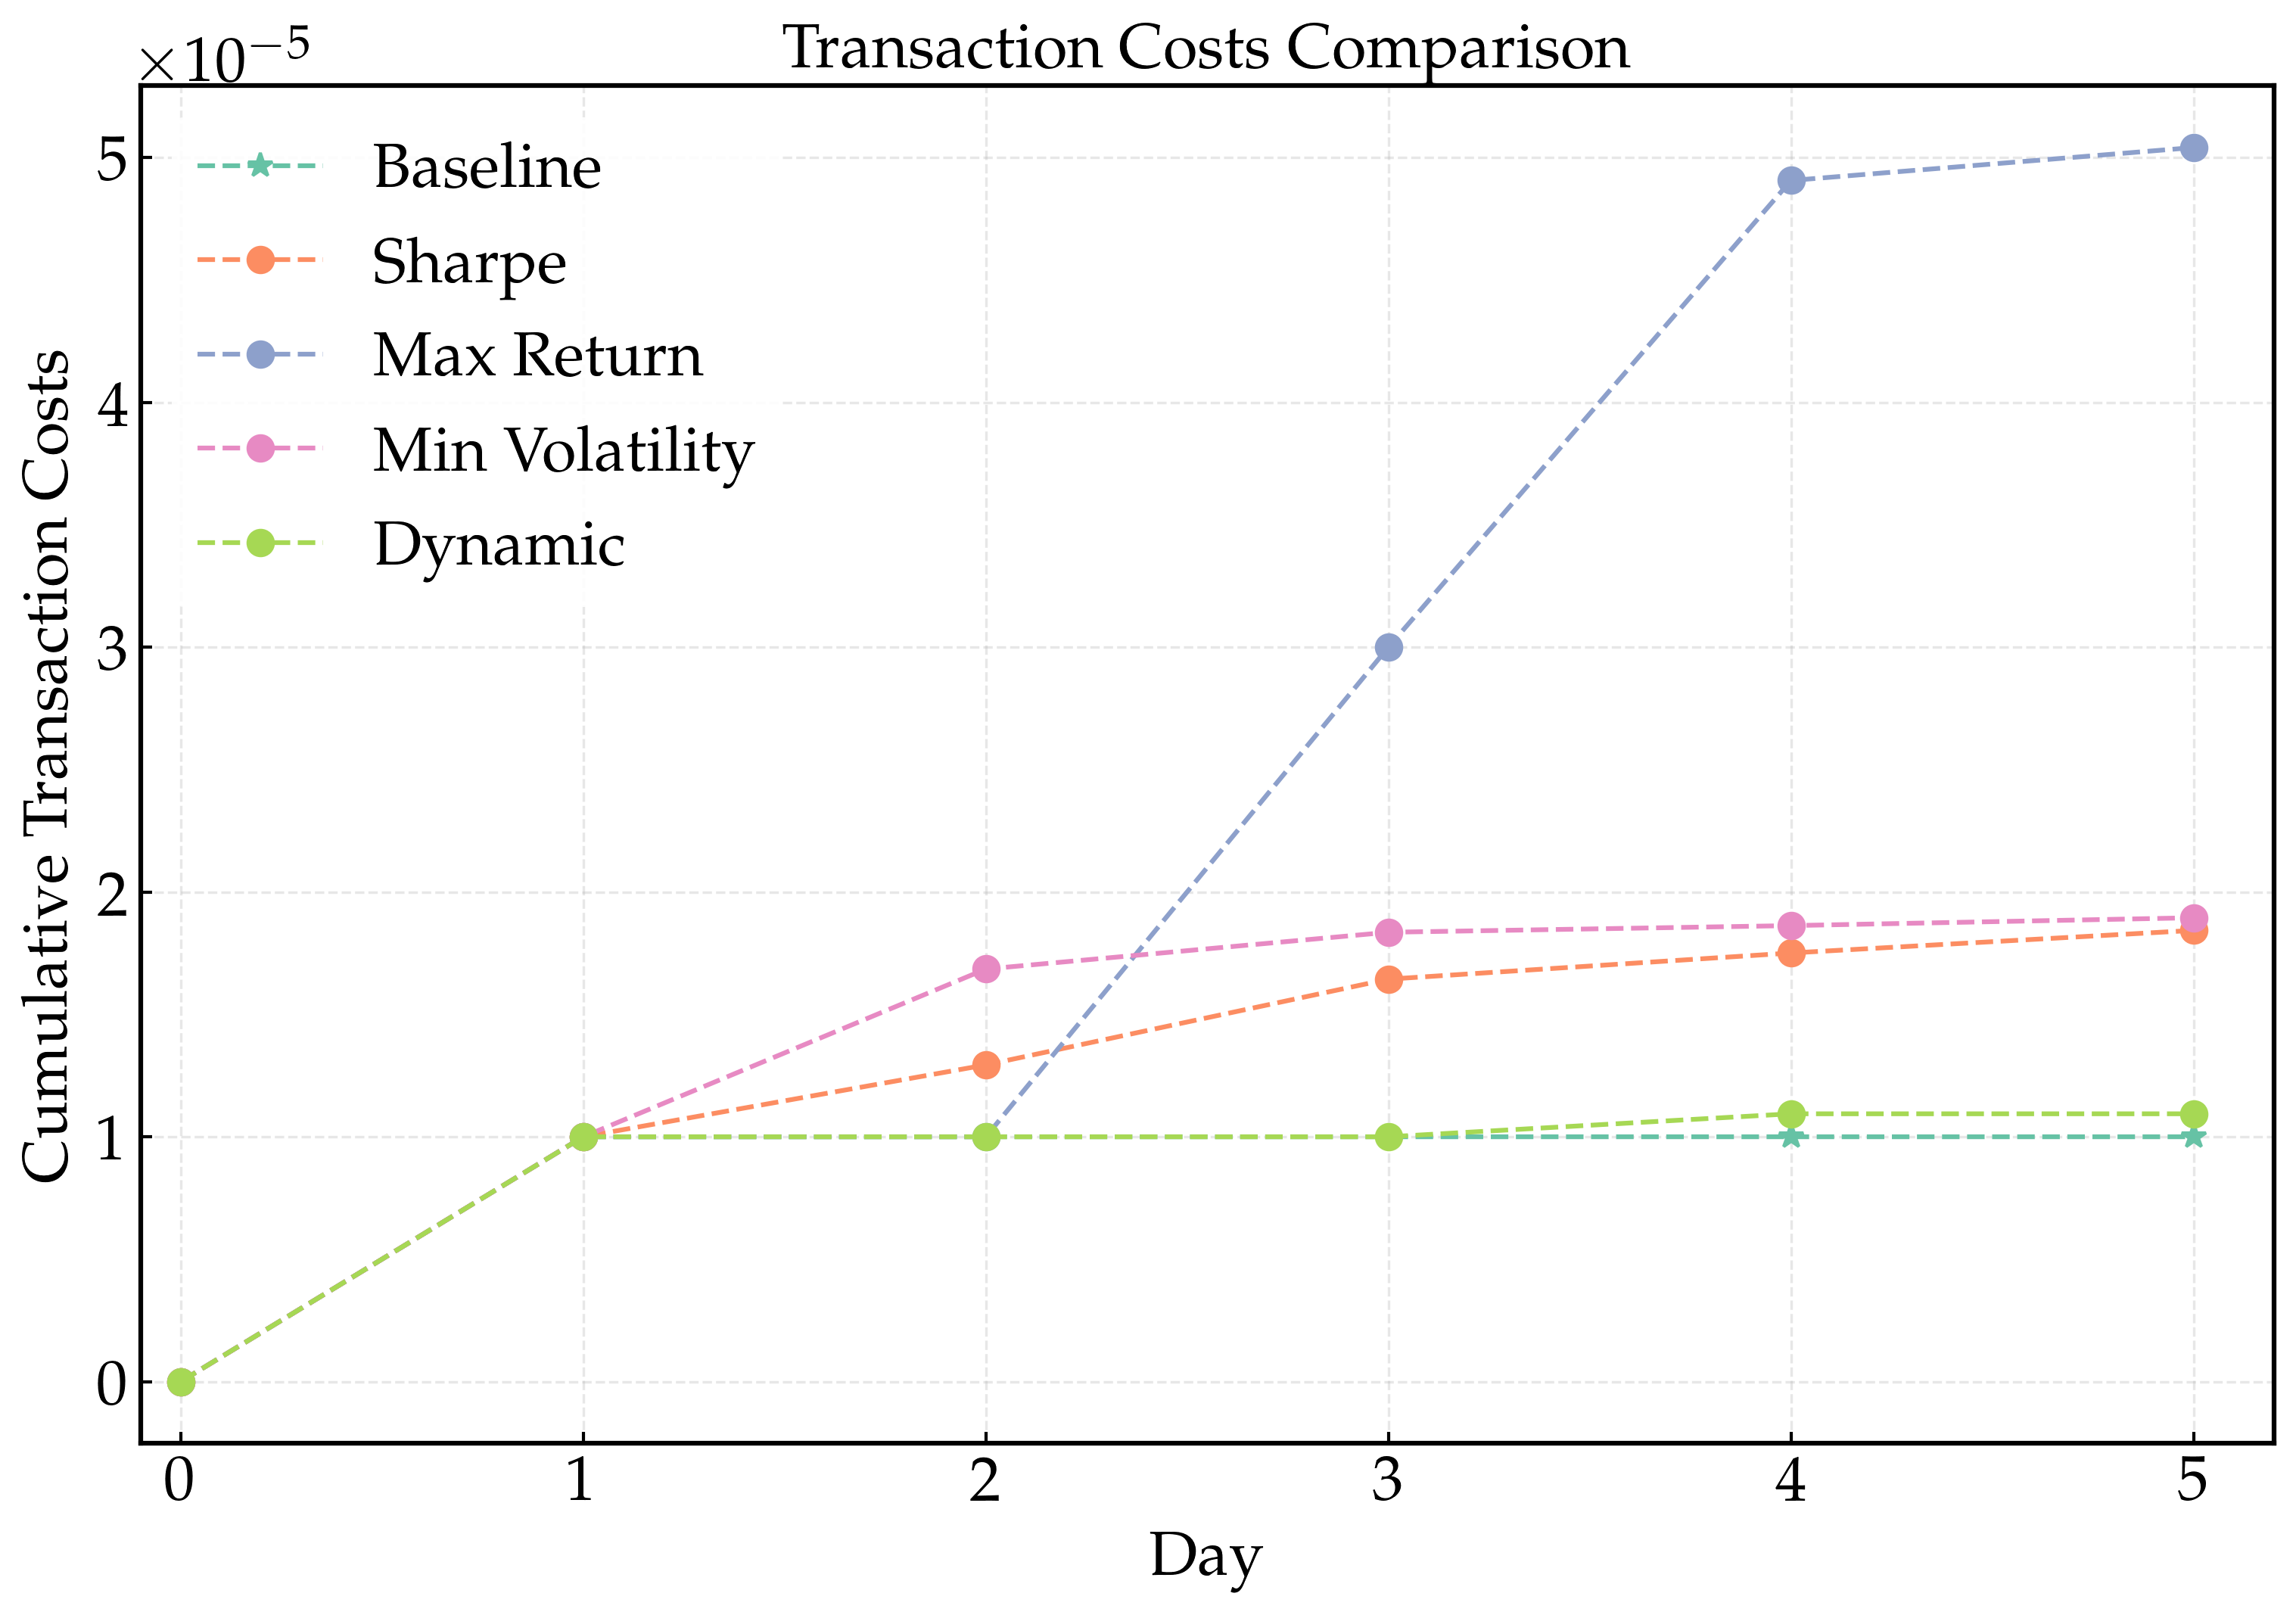
\includegraphics[width=0.6\textwidth]{figures/trx_costs_comparison_final_non.png}
    \caption{Transaction Costs Comparison}
    \label{fig:trx_costs_comparison_non_iterative}
\end{figure}

\paragraph{Implications of Results}

The results underline the significance of incorporating advanced predictive modeling into portfolio optimization. The GPR-based Dynamic Strategy not only demonstrated enhanced performance but also introduced a novel approach to integrating uncertainty into decision-making. By leveraging predictive confidence intervals, the strategy provided a robust mechanism for balancing risk and return, adapting seamlessly to market dynamics.

Moreover, the findings emphasize the critical role of transaction cost management in dynamic portfolio optimization. The reduced costs achieved by the Dynamic Strategy illustrate the potential of intelligent rebalancing mechanisms in improving net returns, a key consideration for practitioners.

\subsubsection{Impact of Iteratively Retrained Models on Strategy Performance}
Other than directly predicting future five days' returns, we also investigate the impact of iteratively retraining the models on the portfolio optimization process. The iterative retraining process aims to adapt the models to changing market conditions by updating the training data with new observations and retraining the models periodically.
 We compare the performance of the iteratively retrained models with the fixed models to evaluate the effectiveness of this approach in enhancing the strategies' adaptability and robustness.
\begin{figure}[htbp]
    \centering
    \includegraphics[width=0.6\textwidth]{figures/iterative/asset_allocations_constant.png}
    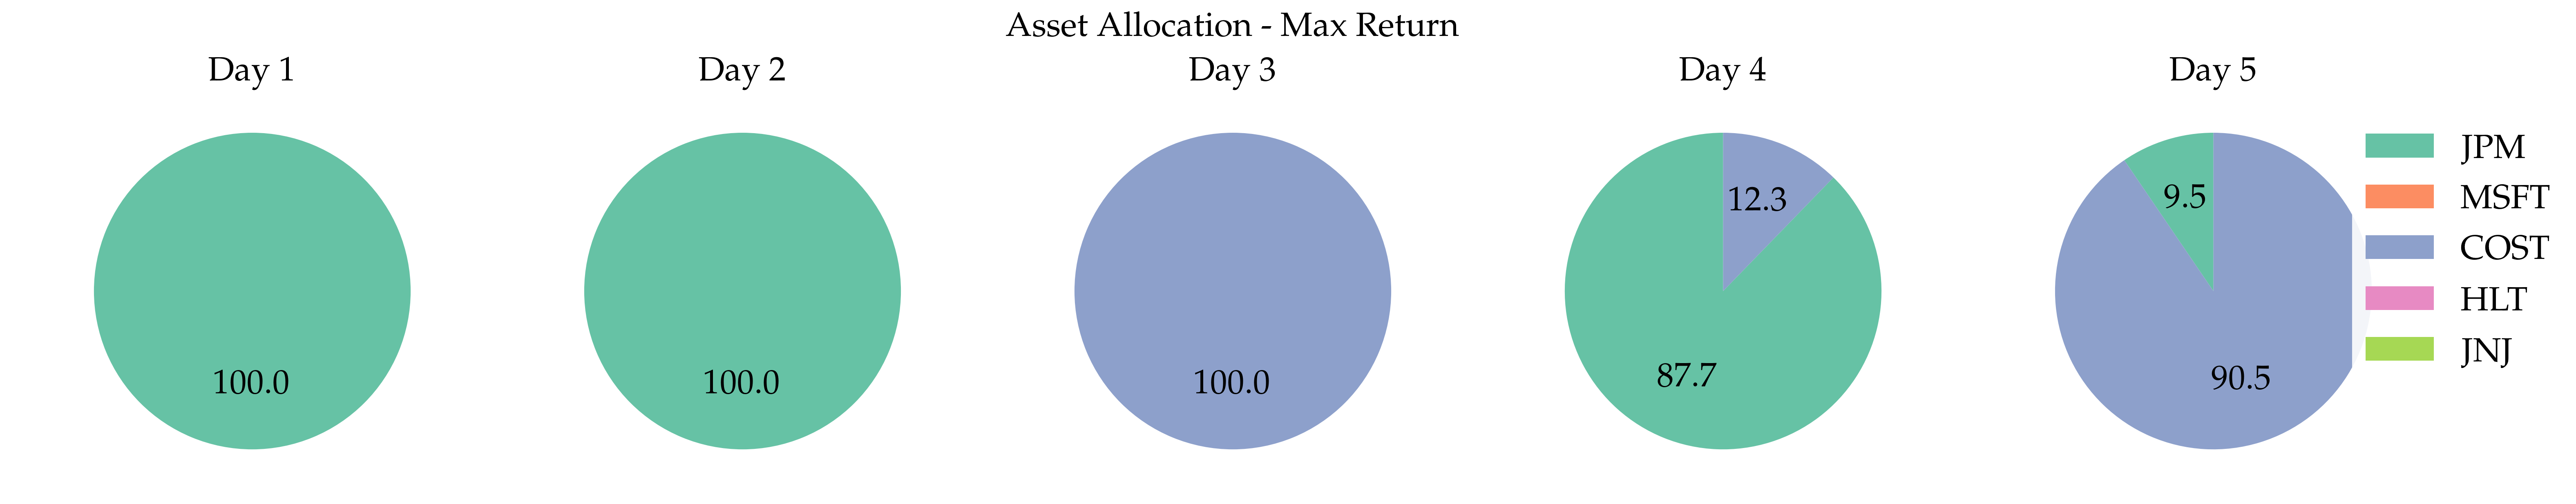
\includegraphics[width=0.6\textwidth]{figures/iterative/asset_allocations_max_return.png}
    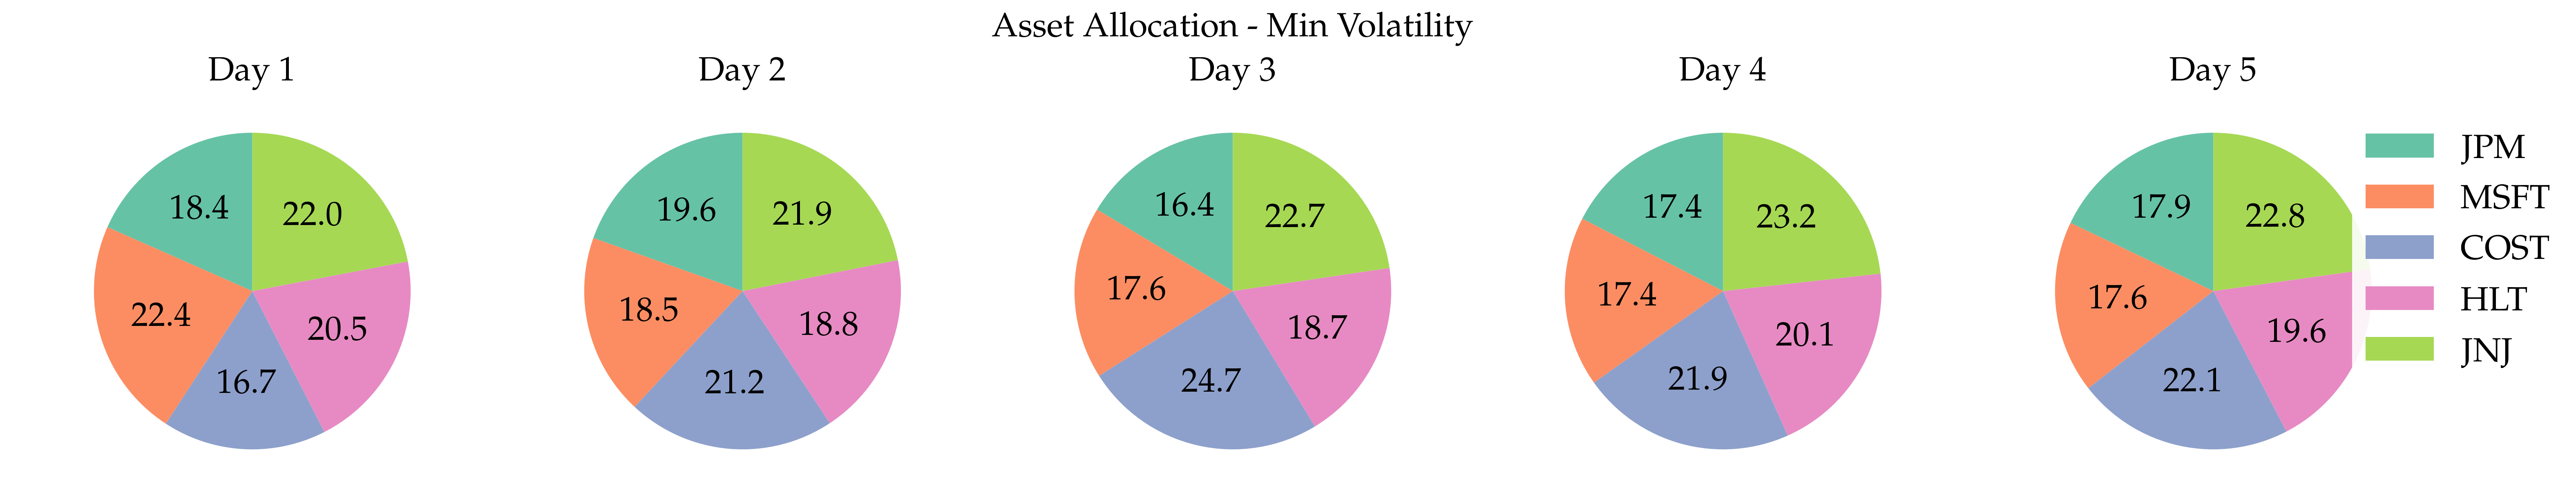
\includegraphics[width=0.6\textwidth]{figures/iterative/asset_allocations_min_volatility.png}
    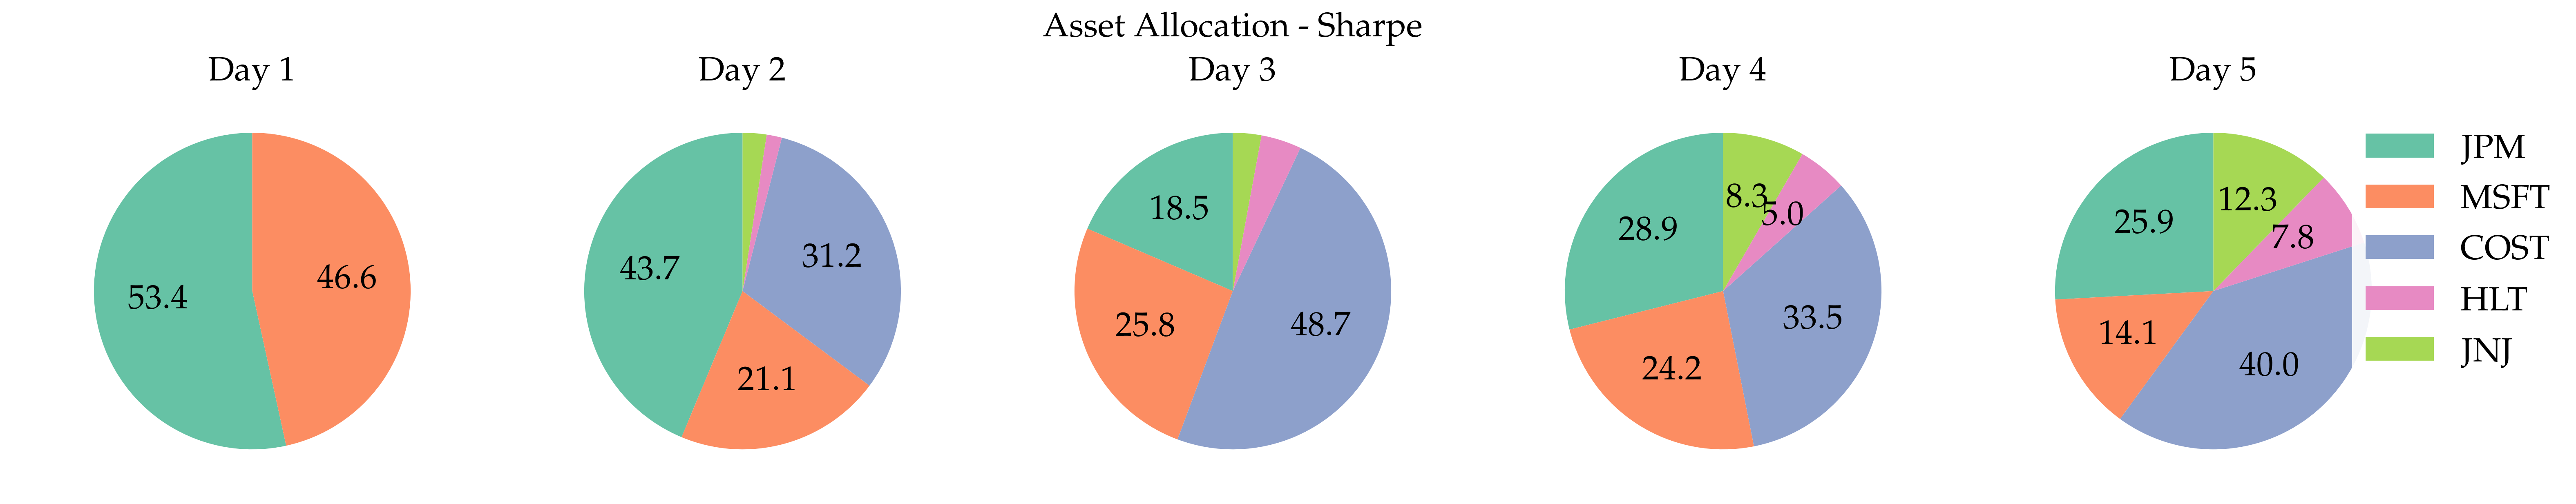
\includegraphics[width=0.6\textwidth]{figures/iterative/asset_allocations_sharpe.png}
    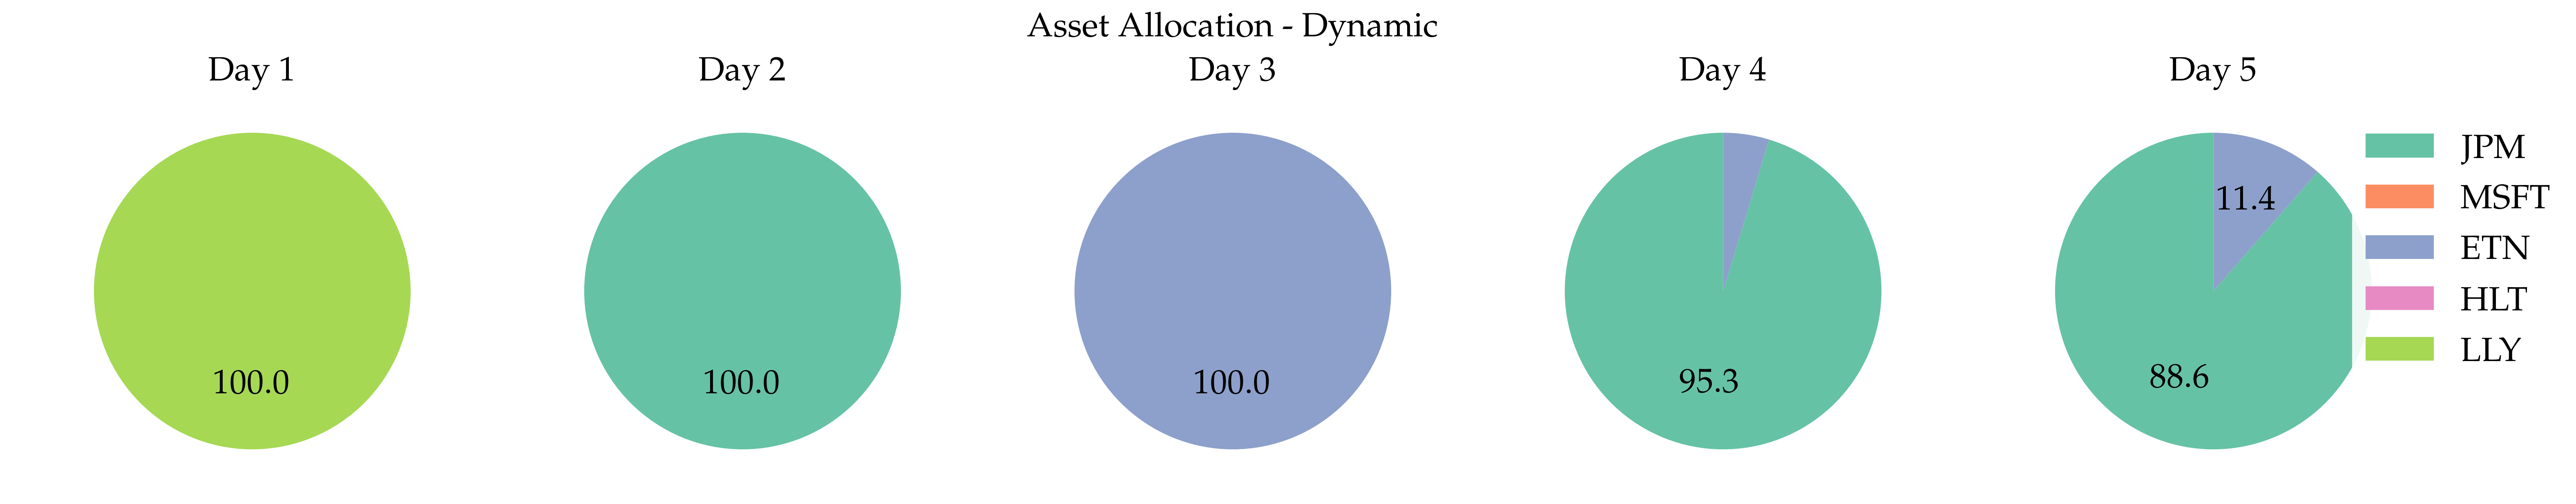
\includegraphics[width=0.6\textwidth]{figures/iterative/asset_allocations_dynamic.png}
    \caption{Portfolio Allocation Evolution of Iteratively Retrained Models}
    \label{fig:asset_allocations_evolution_iterative}
\end{figure}
\begin{figure}[htbp]
    \centering
    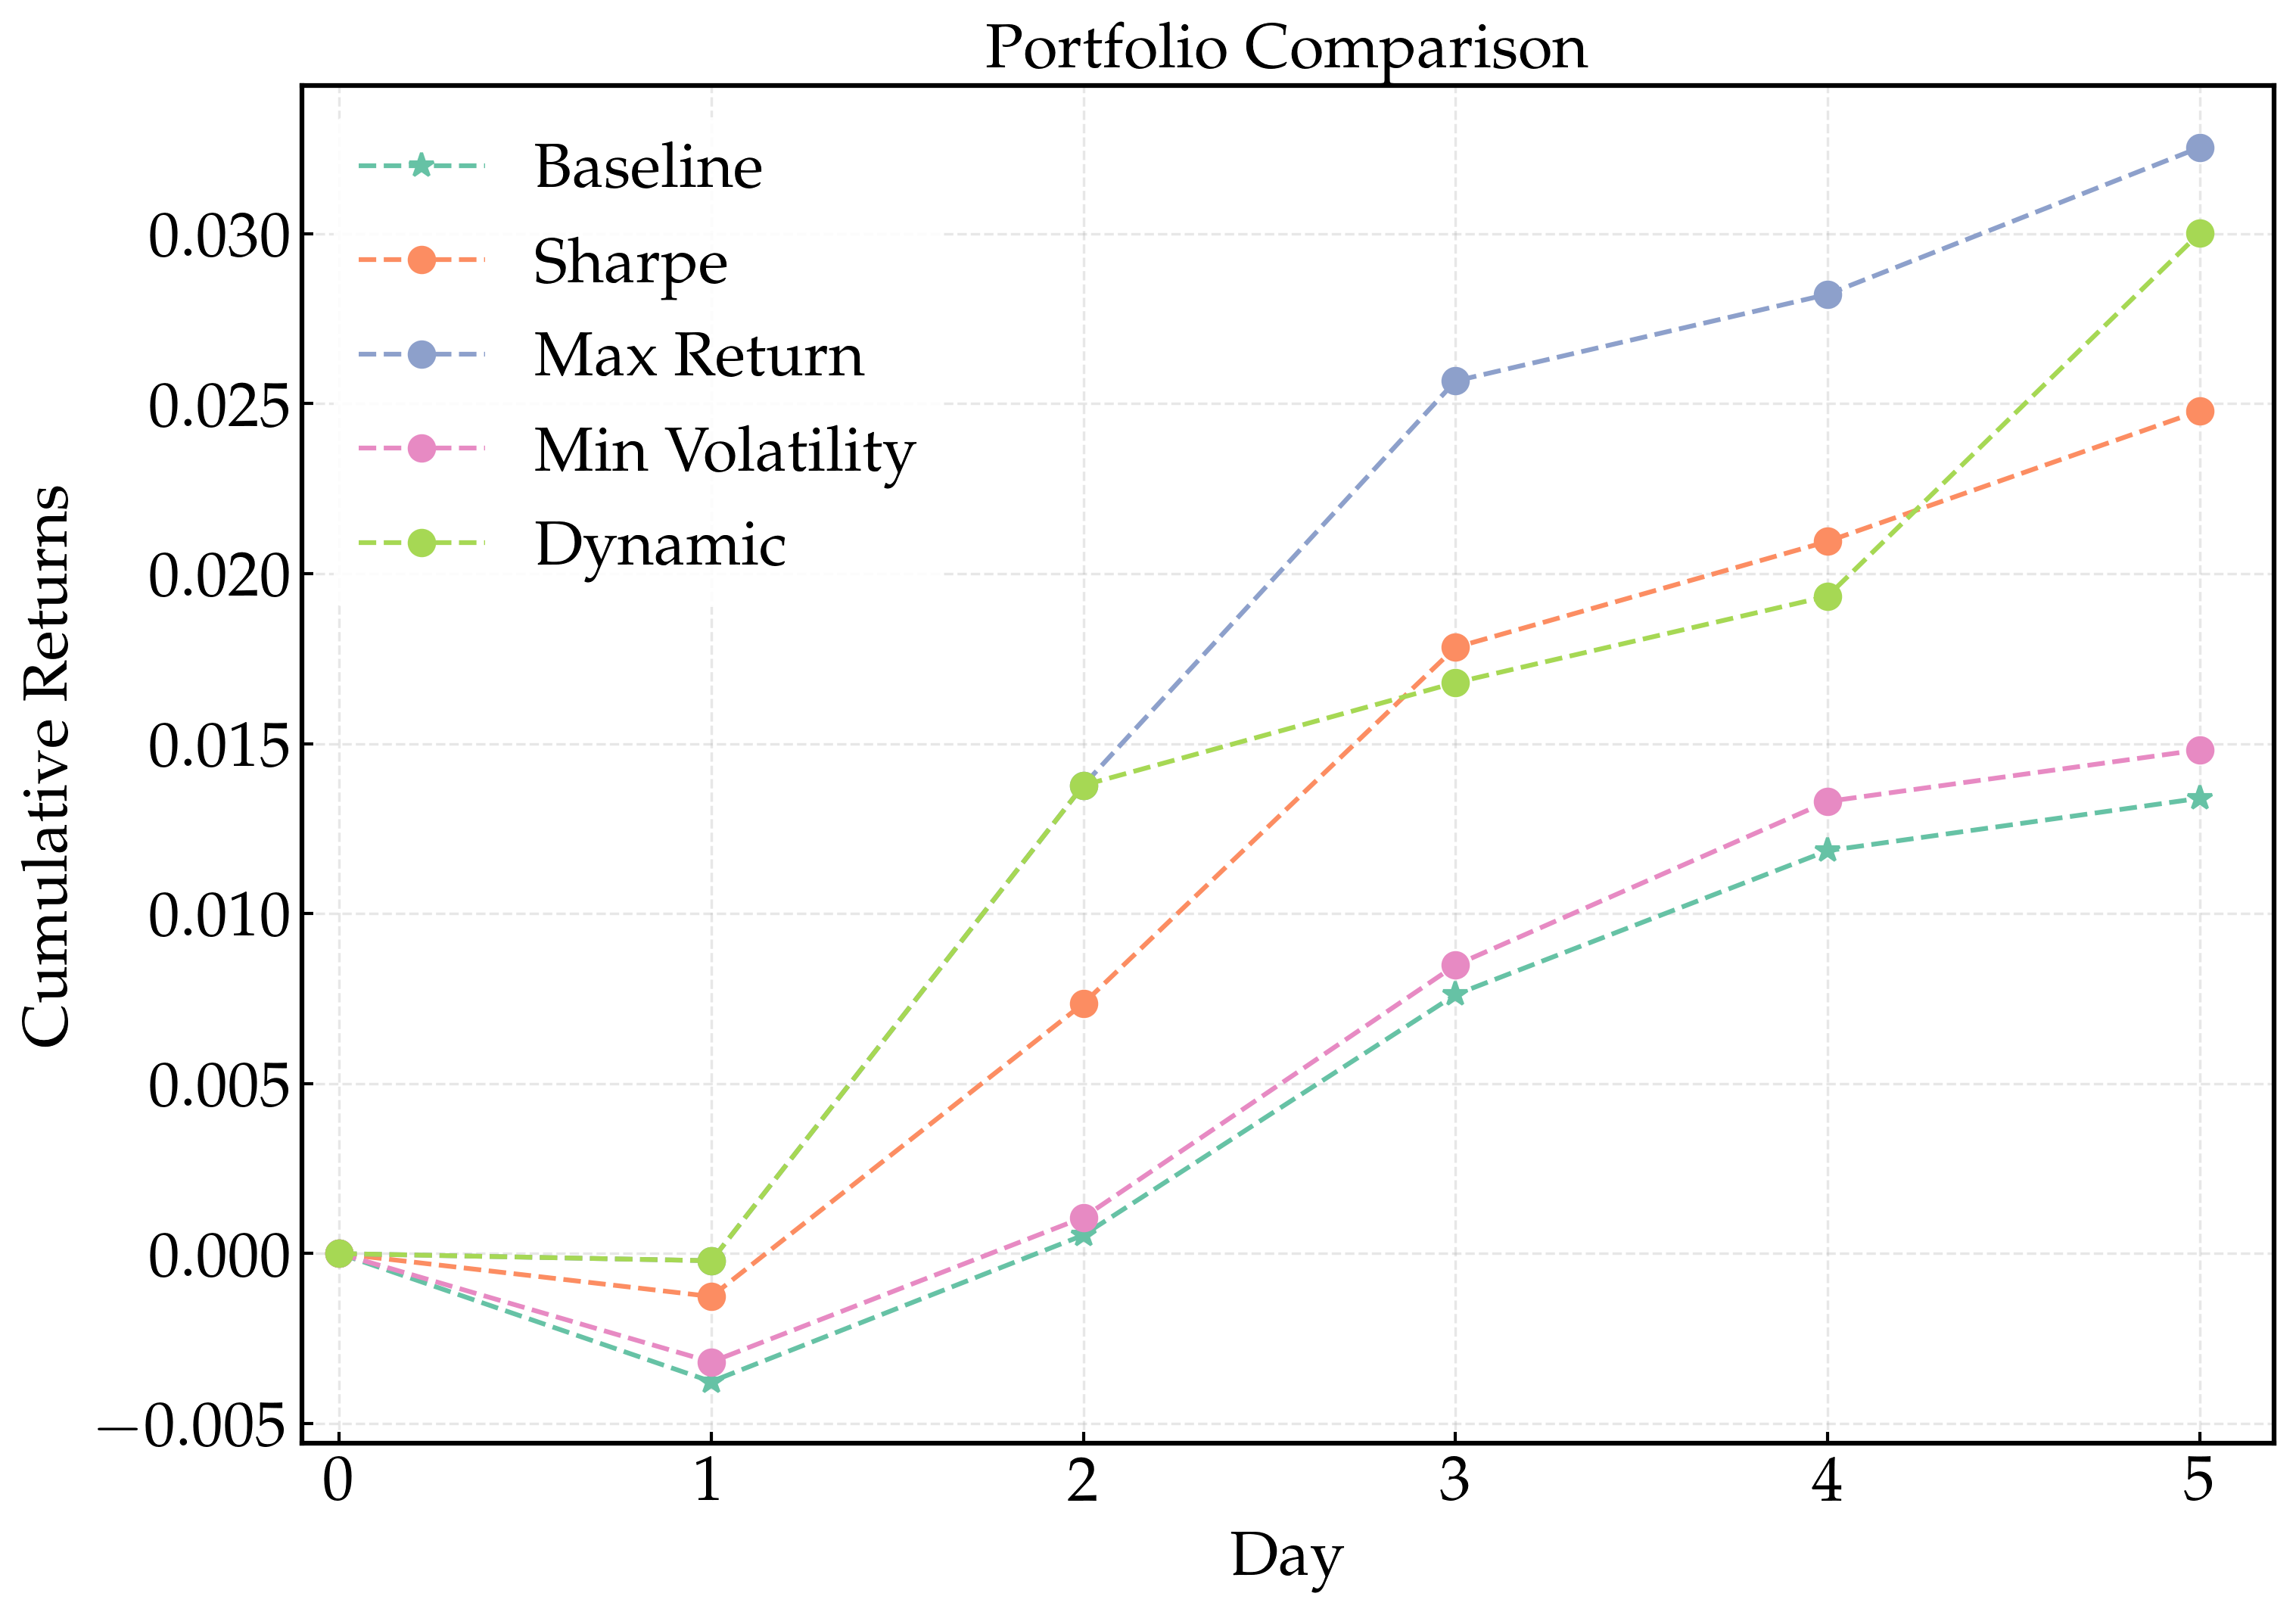
\includegraphics[width=0.6\textwidth]{figures/portfolio_comparison_final.png}
    \caption{Portfolio Comparison of Iteratively Retrained Models}
    \label{fig:portfolio_comparison_iterative}
\end{figure}


\begin{figure}[htbp]
    \centering
    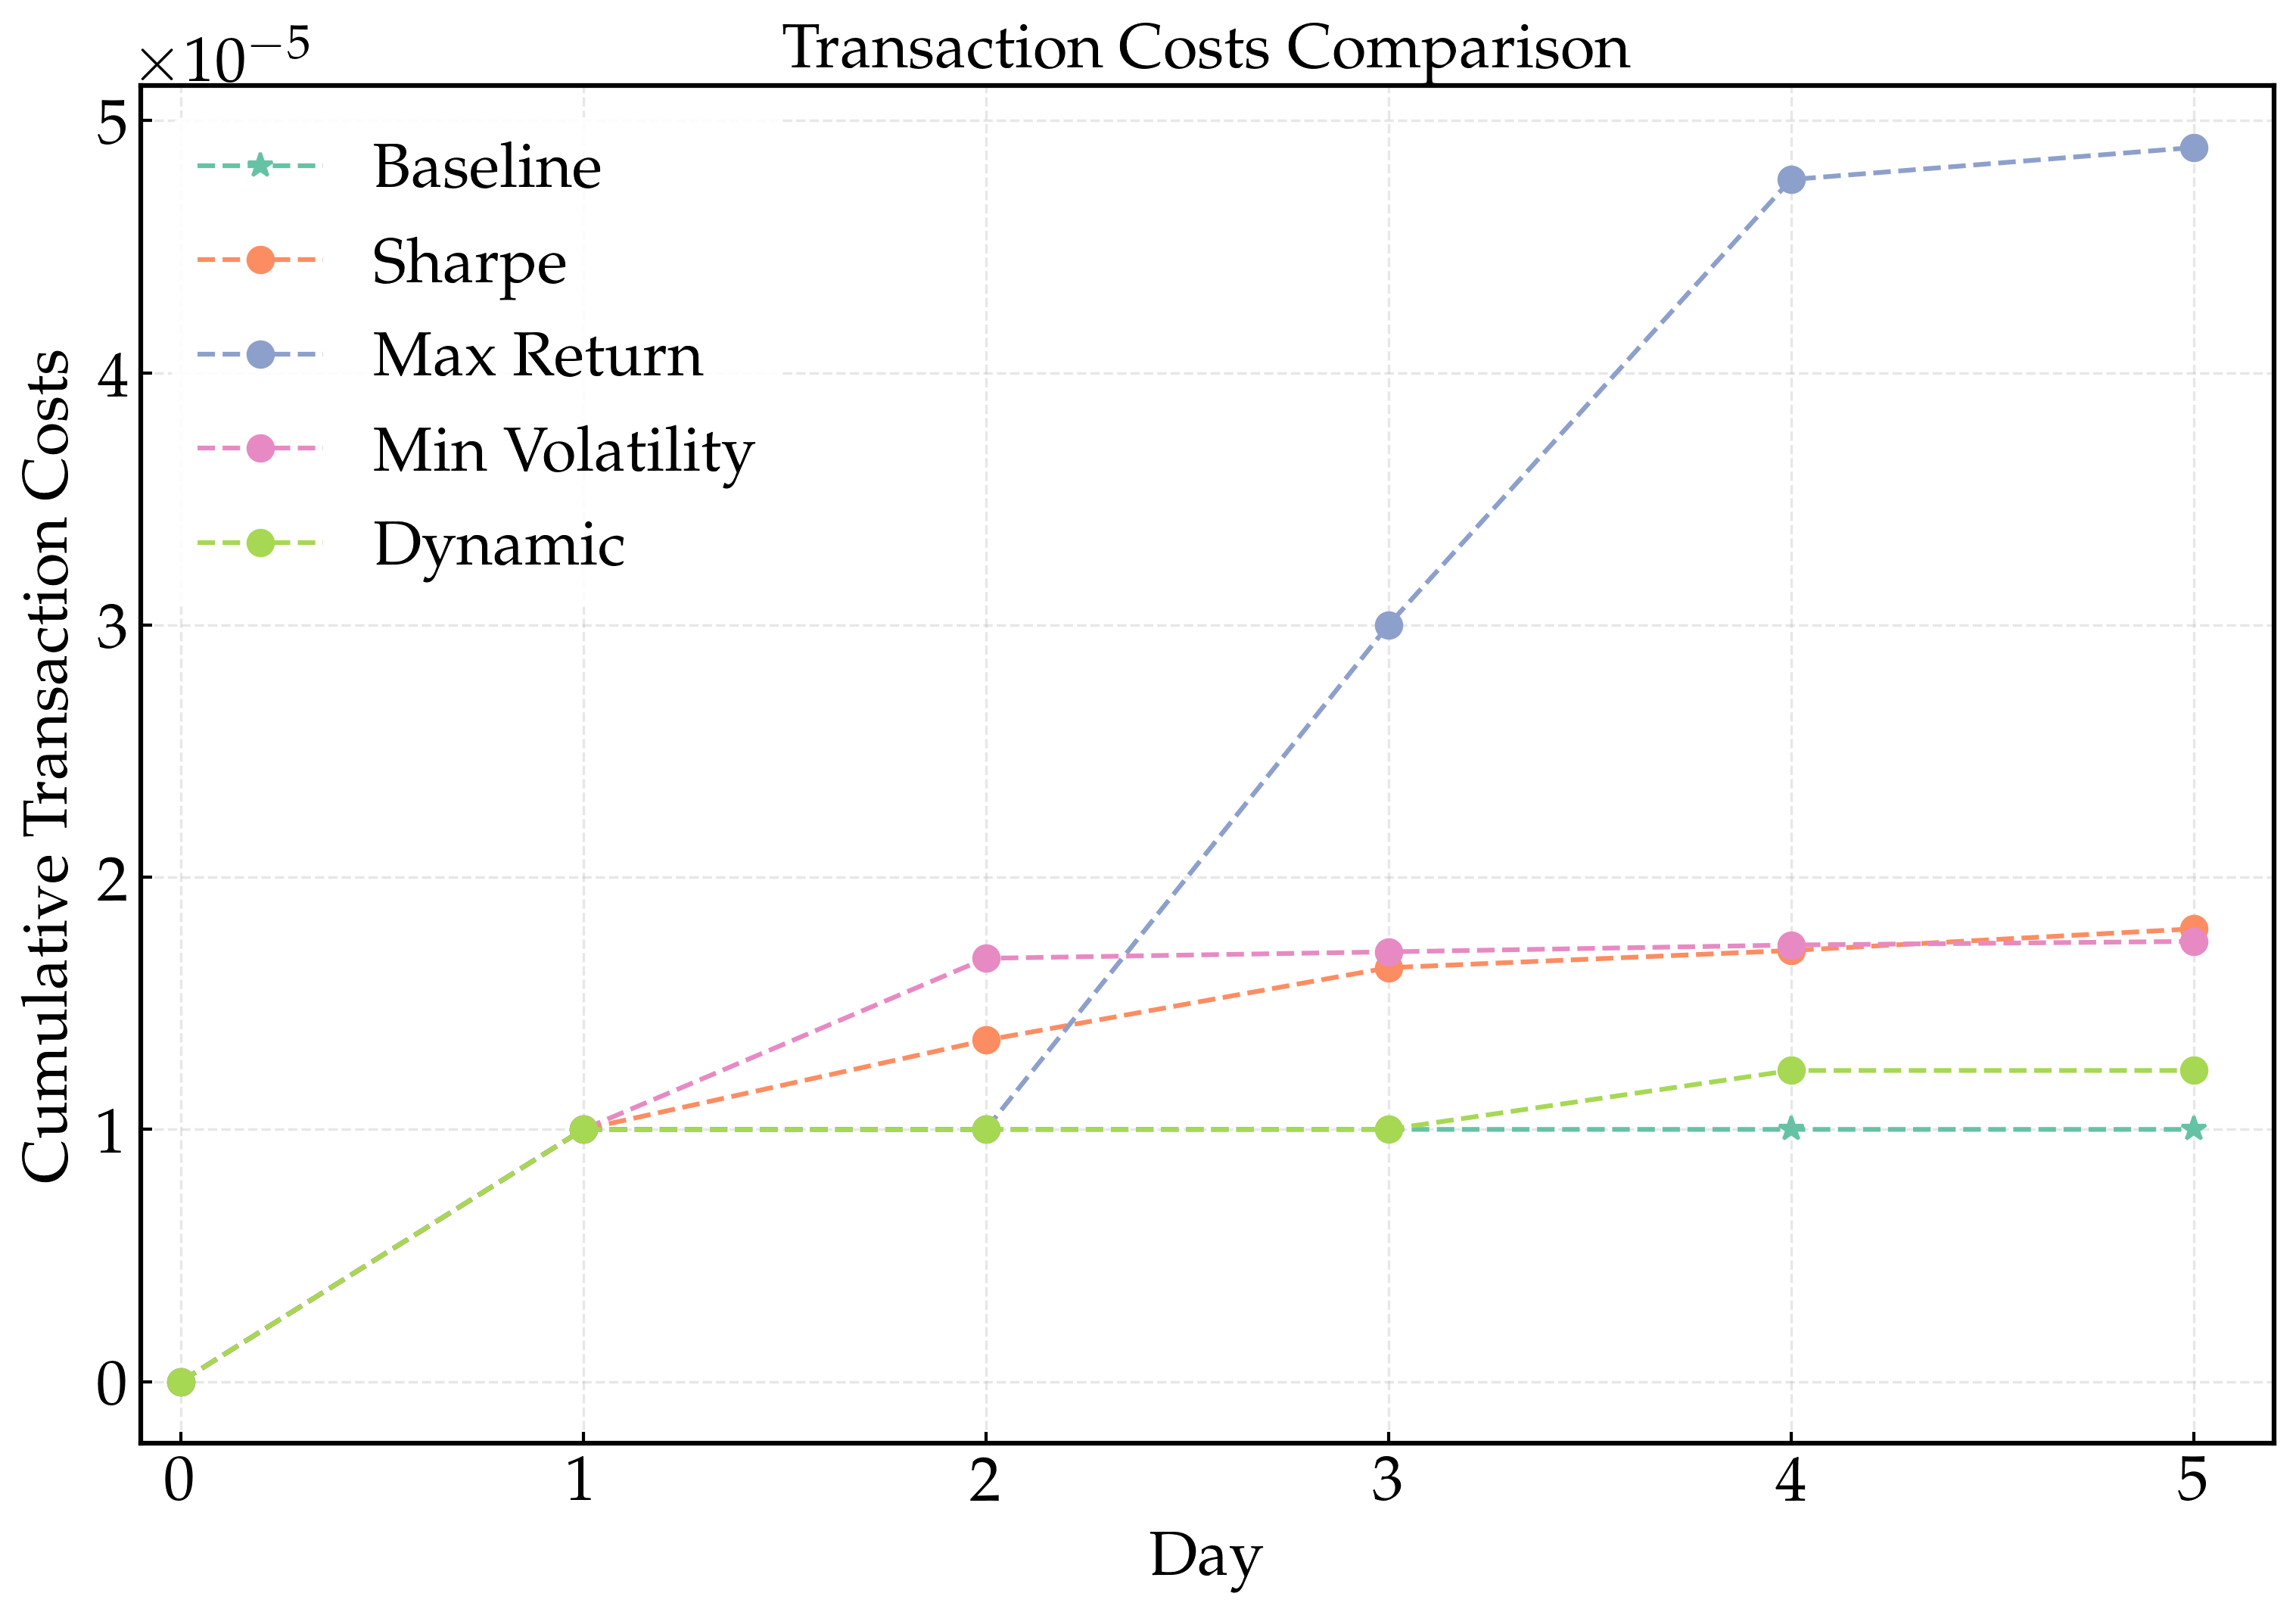
\includegraphics[width=0.6\textwidth]{figures/trx_costs_comparison_final.png}
    \caption{Transaction Costs Comparison of Iteratively Retrained Models}
    \label{fig:trx_costs_comparison_iterative}
\end{figure}

From the plots, we are surpringly to see that the iteratively retrained models have only trivial impact on the strategy performance, which even got less cumulative portfolio returns in backtesting. The iterative retraining process helps the models adapt to changing market conditions, which in this case, the optimizer thinks the market is going down, leading to the dynamic strategy to consistently follow Max Return Strategy. The reduced transaction costs in the iterative approach also indicate that the strategies are more stable and require fewer adjustments over time.

We suspect that the iterative retraining process didn't get a better result in the portfolio optimisation process because the prediction model has large fluctuations when predicting short-term results, whereas it would stablize after two or three days. This is a common issue in financial time series prediction, and we will further investigate this in the future work.



